\documentclass{VUMIFInfKursinis}
\usepackage{algorithmicx}
\usepackage{algorithm}
\usepackage{algpseudocode}
\usepackage{amsfonts}
\usepackage{amsmath}
\usepackage{bm}
\usepackage{color}
\usepackage{graphicx}
% \usepackage{hyperref}  % Nuorodų aktyvavimas
\usepackage{url}


% Titulinio aprašas
\university{Vilniaus universitetas}
\faculty{Matematikos ir informatikos fakultetas}
\institute{Informatikos institutas}  % Užkomentavus šią eilutę - institutas neįtraukiamas į titulinį
\department{Informatikos katedra}
\papertype{Operacinių sistemų pirmoji užduotis}
\title{Multiprograminės OS projektas}
%\titleineng{Modeling of Risk Management Process}
\status{3 kurso 1 grupės studentas}
\author{Dominykas Marma}
% \secondauthor{Vardonis Pavardonis}   % Pridėti antrą autorių
\supervisor{Mantas Grubliauskis}
\date{Vilnius \\ \the\year}

% Nustatymai
% \setmainfont{Palemonas}   % Pakeisti teksto šriftą į Palemonas (turi būti įdiegtas sistemoje)
\bibliography{bibliografija} 

\begin{document}
\maketitle

\tableofcontents

\section{Procesai}

Procesai - vykdomosios programos su esamomis registrų reikšmėmis ir savo kintamaisiais.

\subsection{Procesų būsenos}

\begin{itemize}
	\item Vykdomas - turi procesorių.
	\item Pasiruošęs - vienintelis trūkstamas resursas yra procesorius.
	\item Blokuotas - prašo resųrso (išskyrus procesorių).
	\item Pasiruošęs sustabdytas
	\item Blokuotas sustabdytas
\end{itemize}

\subsection{Planuotojas}

Planuotojo paskirtis - atimti procesorių iš procceso, peržvelgti pasiruošųsių procesų sąrašą ir paduoti procesorių tinkamiausiam iš jų.

\subsubsection{Prioritetai}

Visi procesai turi prioritetus nuo 0 iki 20, kuo didesnis prioritetas, tuo didesnė tikimybė, kad procesas bus vykdomas.

\subsection{Procesų primityvai}

\begin{itemize}
	\item Kurti procesą - perduodama nuoroda į tėvą, p
	\item Naikinti procesą
	\item Stabdyti procesą
\end{itemize}

\subsection{Procesų kūrimo ir trynimo lentelė}

\begin{table}[H]\footnotesize
	\centering
	\caption{Procesų kūrimo ir trynimo lentelė}    % Antraštė įterpiama prieš lentelę
	\begin{tabular}{|c|c|c|}
		\hline
		Proceso pavadinimas & Procesas, kuris jį sukuria & Procesas, kuris jį ištrina \\
		\hline
		StartStop & Niekas (sistemos pradžioje pasileidžia) & Niekas (pats išsijungia) \\
		\hline
		ReadFromInterface & StartStop & StartStop\\
		\hline
		JCL & StartStop & StartStop \\
		\hline
		MainProc & StartStop & StartStop \\
		\hline
		Loader & StartStop & StartStop \\
		\hline
		JobGovernor & MainProc & MainProc \\
		\hline
		VirtualMachine & JobGovernor & JobGovernor \\
		\hline
		Interrupt & StartStop & StartStop \\
		\hline
		PrintLine & StartStop & StartStop \\
		\hline
	\end{tabular}
	\label{tab:duomenys}
\end{table}

\subsection{StartStop}

Paskirtis - darbo pradžioje sukurti resursus ir sisteminius procesus.

\begin{figure}[H]
	\centering	
	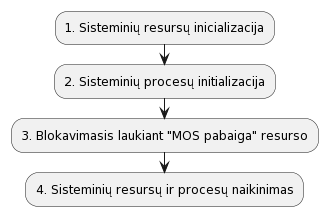
\includegraphics[scale=0.65]{img/StartStop}
	\caption{Proceso StartStop diagrama}   % Antraštė įterpiama po paveikslėlio
	\label{img:StartStop}
\end{figure}

\subsection{ReadFromInterface}

Paskirtis - gavus informaciją iš įvedimo srauto atlikti pirminį jos apdorojimą, atiduoti informaciją procesui JCL, tolesniam apdorojimui.

\begin{figure}[H]
	\centering	
	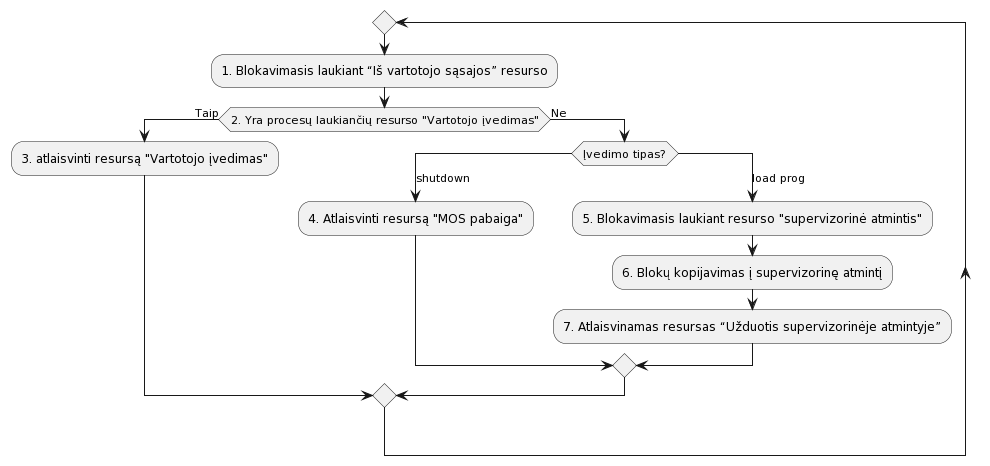
\includegraphics[scale=0.65]{img/ReadFromInterface}
	\caption{Proceso StartStop diagrama}   % Antraštė įterpiama po paveikslėlio
	\label{img:ReadFromInterface}
\end{figure}

\subsection{JCL}

JCL paskirtis - patikrinti perkeltos programos korektiškumą.

\begin{figure}[H]
	\centering	
	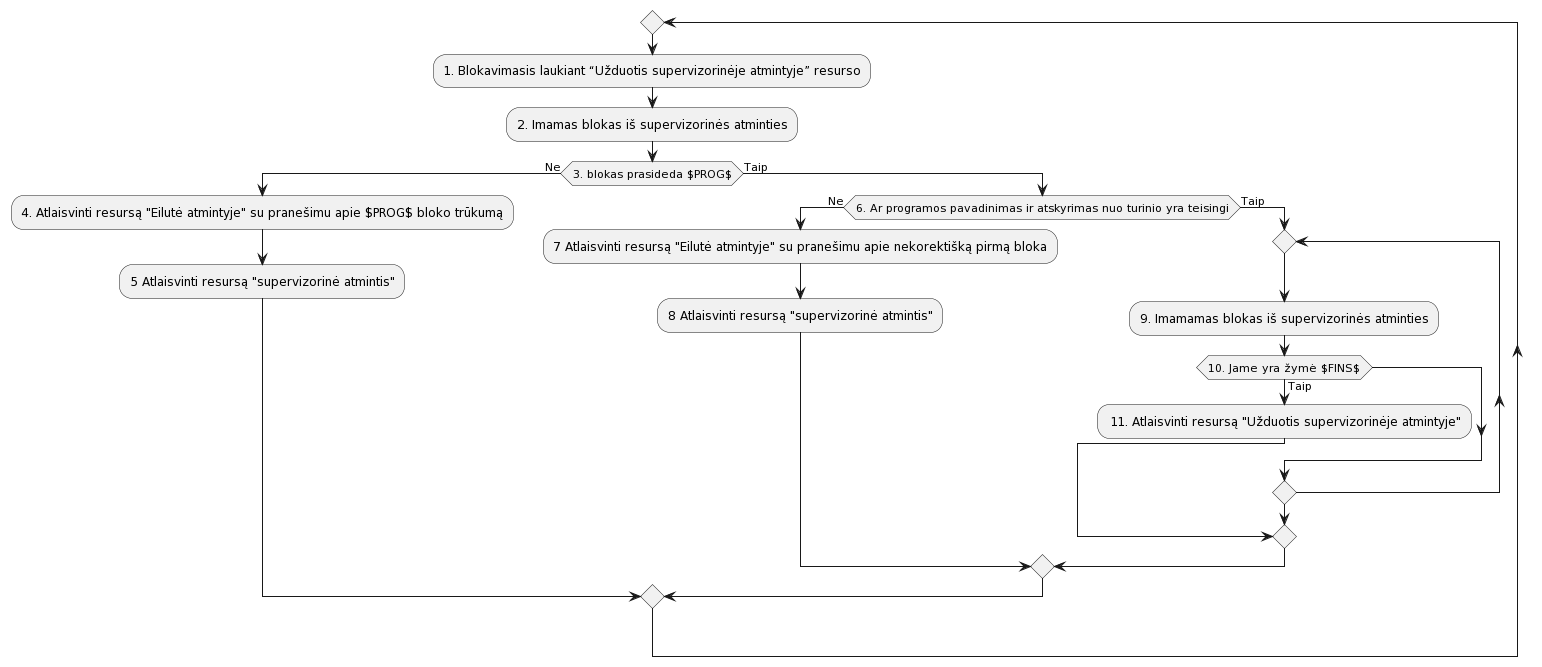
\includegraphics[scale=0.3]{img/JCL}
	\caption{Proceso JCL diagrama}   % Antraštė įterpiama po paveikslėlio
	\label{img:JCL}
\end{figure}

\subsection{MainProc}

MainProc paskirtis - kurti ir naikinti procesus JobGovernor.

\begin{figure}[H]
	\centering	
	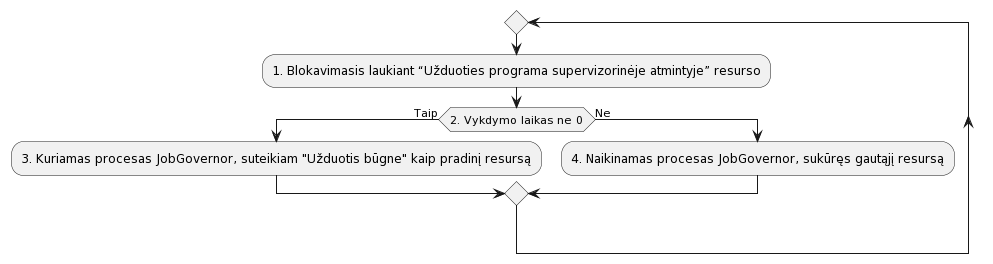
\includegraphics[scale=0.40]{img/MainProc}
	\caption{Proceso MainProc diagrama}   % Antraštė įterpiama po paveikslėlio
	\label{img:MainProc}
\end{figure}

\subsection{Loader}

Loader paskirtis - perkelti blokus iš išorinės atminties į vartotojo atmintį.

\begin{figure}[H]
	\centering	
	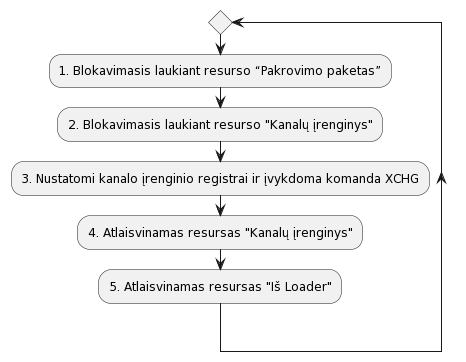
\includegraphics[scale=0.65]{img/Loader}
	\caption{Proceso Loader diagrama}   % Antraštė įterpiama po paveikslėlio
	\label{img:Loader}
\end{figure}

\subsection{JobGovernor}

JobGovernor paskirtis - kurti, naikinti VIrtualMachine ir padėti tvarkyti pertraukimus.

\begin{figure}[H]
	\centering	
	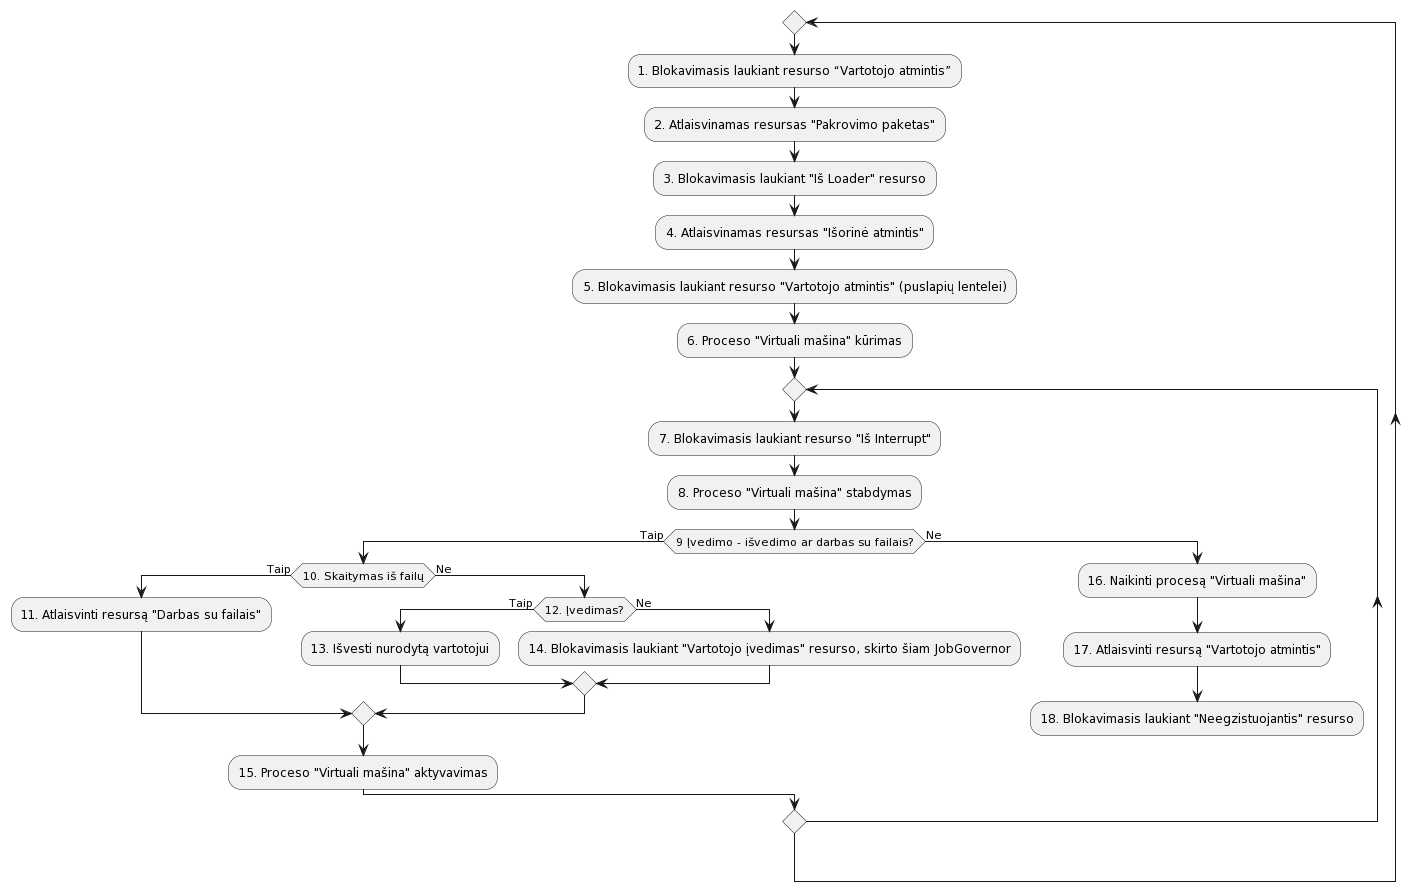
\includegraphics[scale=0.3]{img/JobGovernor}
	\caption{Proceso JobGovernor diagrama}   % Antraštė įterpiama po paveikslėlio
	\label{img:JobGovernor}
\end{figure}

\subsection{VirtualMachine}

VirtualMachine paskirtis - vykdyti vartotojo užduoties programą.

\begin{figure}[H]
	\centering	
	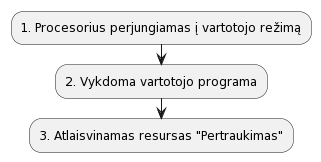
\includegraphics[scale=0.65]{img/VirtualMachine}
	\caption{Proceso VirtualMachine diagrama}   % Antraštė įterpiama po paveikslėlio
	\label{img:VirtualMachine}
\end{figure}

\subsection{Interrupt}

Proceso Interrupt paskirtis - reaguoti į pertraukimus, kilusius virtualios mašinos darbo metu.

\begin{figure}[H]
	\centering	
	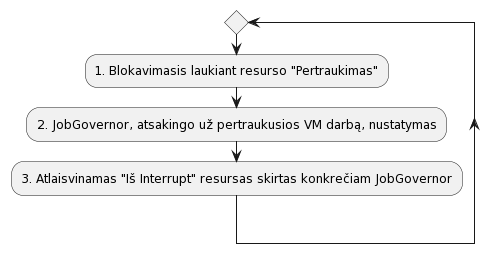
\includegraphics[scale=0.65]{img/Interrupt}
	\caption{Proceso Interrupt diagrama}   % Antraštė įterpiama po paveikslėlio
	\label{img:Interrupt}
\end{figure}

\subsection{PrintLine}

Proceso PrintLine paskirtis - į išvedimo srautą pasiųsti pranešimą.

\begin{figure}[H]
	\centering	
	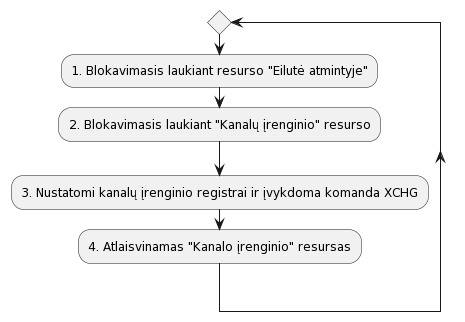
\includegraphics[scale=0.65]{img/PrintLine}
	\caption{Proceso PrintLine diagrama}   % Antraštė įterpiama po paveikslėlio
	\label{img:PrintLine}
\end{figure}

\subsection{FileSystem}

(darbus su failais turėtų nurodyti informaciją)

?Kaip virtualiai mašinai nustato registrus?

Proceso paskirtis - aptarnauti veiksmus, susijusius su failų sistema.

\begin{figure}[H]
	\centering	
	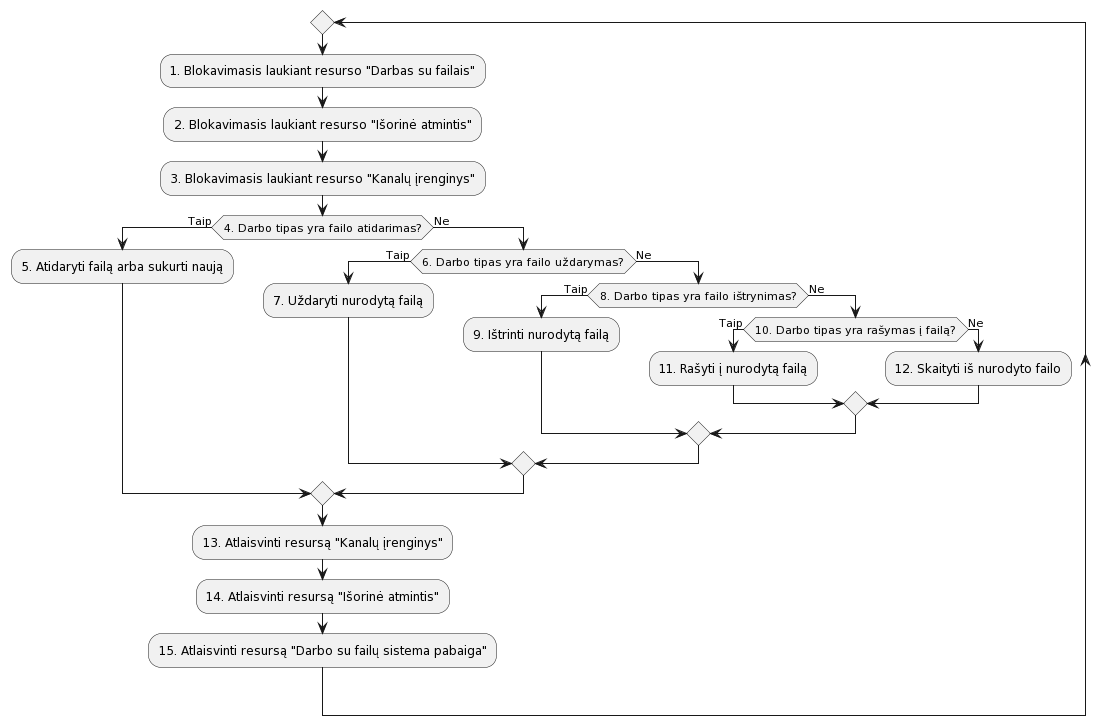
\includegraphics[scale=0.35]{img/FileSystem}
	\caption{Proceso FileSystem diagrama}   % Antraštė įterpiama po paveikslėlio
	\label{img:FileSystem}
\end{figure}

\subsection{Idle}

Proceso Idle paskirtis - būti vykdomam, kai nėra kitų pasiruošusių procesų.

\begin{figure}[H]
	\centering	
	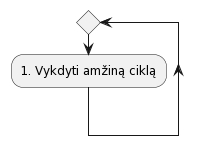
\includegraphics[scale=0.65]{img/Idle}
	\caption{Proceso Idle diagrama}   % Antraštė įterpiama po paveikslėlio
	\label{img:Idle}
\end{figure}


\section{Resursai}

\subsection{Resursų lentelė}

% https://tex.stackexchange.com/questions/40561/table-with-multiple-lines-in-some-cells
% p prie parametrų turbūt, kad būtų multiline
\begin{table}[H]\footnotesize
	\centering
	\caption{Resursų lentelė}    % Antraštė įterpiama prieš lentelę
	\begin{tabular}{|c|c|c|c|}
		\hline
		Resurso pavadinimas & Resursą kuria & Resursą atlaisvina & Dėl resurso blokuojasi \\
		\hline
		\multicolumn{4}{c}{SISTEMINIAI}\\
		\hline
		Kanalų įrenginys & ------- & Loader, PrintLine & Loader, PrintLine\\
		\hline
		Supervizorinė atmintis & ------- & & ReadFromInterface \\
		\hline
		Vartotojo atmintis & ------- & & JobGovernor\\
		\hline
		Išorinė atmintis & ------- & JobGovernor & JobGovernor \\
		\hline
		\multicolumn{4}{c}{PROGRAMINIAI}\\
		\hline
		Užduotis būgne & & JCL & MainProc \\
		\hline
		MOS pabaiga & & & StartStop \\
		\hline
		Iš vartotojo sąsajos &  & & ReadFromInterface \\
		\hline
		Užduotis supervizorinėje atmintyje & & ReadFromInterface & JCL \\
		\hline
		Užduotis būgne & & JCL & MainProc \\
		\hline
		Pakrovimo paketas & & JobGovernor & Loader \\
		\hline
		Iš Loader & & Loader & JobGovernor \\
		\hline
		Eilutė atmintyje & & JCL & PrintLine\\
		\hline
		Iš Interrupt & & Interrupt & JobGovernor\\
		\hline
		Vartotojo įvedimas & & & JobGovernor \\
		\hline 
		Pertraukimas & & VirtualMachine & Interrupt\\
		\hline 
		Darbas su failais & StartStop & JobGovernor & FileSystem \\
		\hline
		Neegzistuojantis & StartStop & ------- & JobGovernor \\
		\hline
	\end{tabular}
	\label{tab:resursu_lentele}
\end{table}

\printbibliography[heading=bibintoc] % Literatūros šaltiniai aprašomi
\appendix  % Priedai

\end{document}
